\section{Methodology}
\label{sec:method}
Before explaining our contributions in detail, we note here that the framework of the \gob\ analyzer had to be adapted, so that the parallelized solvers do not run into concurrency issues. We  protect certain functions with a mutex such that they cannot be called multiple times in parallel. Amongst other examples, this is necessary for functions related to printing output as otherwise multiple messages can get mixed together. Furthermore, we make certain data-structures thread local, meaning, that the worker threads do not share these data-structure, but instead each thread has a local copy of it. For example this applies to the data-structure responsible for timing different parts of the analysis.

  \subsection{Constraint systems with \texttt{create} edges}
  \label{sec:method:create}
  We want to give the solvers hints, which variables can likely be iterated in parallel. As we explained in~\autoref{sec:background:constrSys}, in \gob\ a variable can have a \ac{rhs} that queries a variable but discards the result. This is a suitable location for parallelization, as a variable whose value is not needed anyway can be iterated in parallel to the iterations of the main solver. A sequential solver has to pause the current \ac{rhs} evaluation to compute a to-be-discarded solution for the queried variable, while a parallel solver can continue the \ac{rhs} evaluation while computing a solution for the queried variable in parallel.
  To integrate this idea in our notion of a constraint system, we introduce \texttt{create} edges. \texttt{Create} edges have a target variable $x$. Similar to \texttt{query} edges, they require the solver, to solve the target variable for a satisfying solution. However, they also tell the solver, that the variable that is the origin of this \texttt{create} edge does not depend on the result. Concretely, we introduce \texttt{create} edges at points in the program, where a thread is created. The target variable is the return-point of the created thread. Thus, it is ensured that a solution for sub-system of the thread is computed.

  \subsection{Lockable Hash-table}
  \label{sec:method:LHM}
  During the solving process, the solvers store and update a mapping of variables to values and track further information about the variables. For this, the existing single-threaded top-down solver uses hash-tables, since it allows for fast access and updates. However, for a multithreaded solver the access to these data-structures has to be guarded by a mutex to allow only a single thread to read and write the information belonging to a variable during a critical section. 
  A straight forward idea is to lock the whole hash-table with a single mutex. This however takes away much potential for parallel work, since large parts of the solver are spent in critical sections.
  We propose a \textit{lockable hash-table} that splits the mapping it stores into a set number of \textit{n} buckets, where each of the buckets can be locked with a mutex. The bucket, in which the value for a variable is stored is determined by a hash function, e.g. the mapping for variable \textit{x} is stored in bucket $\text{hash}(x)\ \text{mod}\ n$. This allows for parallel work on multiple variables without waiting, as long as these variables are placed in different buckets.

  \subsection{Parallelized top-down solvers}
  \label{sec:method:td_parallel}
  In this section we describe the workings of three different parallel solvers as we implemented them in the \gob\ analyzer. The concepts for these solvers were given to us and discussed in private communication with Helmut Seidl, Michael Schwarz and Ali Rasim Kocal~\cite{privCom}. The basis for all three solvers is the \ac{td} we described in~\autoref{sec:background:td}. We note here that the stealing \ac{td} does not use the \texttt{create} edges we introduced in~\autoref{sec:method:create}, while the shared-memory \ac{td} and the disjunct \ac{td} need these edges to perform work in parallel.

    \subsubsection{Stealing TD}
    \label{sec:method:td_parallel:stealing}
    The idea of the stealing \ac{td} is to start multiple \acp{td} in parallel. The hope is that they find different spots in the constraint system where multiple iterations are needed. The parallel solvers work independently of each other but have a shared data-structure for the value of the variables and tracking which variables are called and which are stable. If one solver at some point queries a variable that was already iterated by another one, it can use the result from that solver. These variables are then \textit{stolen} from the solver that worked on them previously.
    For this concept to work, the solvers are organized in a hierarchy. Thus, each solver has a distinct \ac{prio} with higher prioritized solvers stealing variables from lower prioritized solvers. Furthermore, the concept of calledness and stability changes for the stealing \ac{td}. A variable is no longer either called or uncalled, but it is assigned a called-\ac{prio} coinciding with the \ac{prio} of the solver that \textit{owns} it, with a special value indicating, that a variable is not owned at all. Solvers take ownership of a variable when they first encounter it during a query and it is not owned by a higher prioritized solver. If the variable is assigned a lower called-\ac{prio}, the solver \textit{steals} it, if not, the solver marks the variable as a wpoint and uses its current value.
    After finding a stable solution for a variable, the solver gives up ownership of that variable. It is not given back to a solver from which it was stolen, instead it is not owned by any solver at all. Similarly, variables are assigned a stable-\ac{prio} according to the solver that computed the stable value. Solvers see variables with their own or a higher stable-\ac{prio} as stable, but variables with a lower stable-\ac{prio} as unstable and iterate those again. If a variable gets stolen from a solver during a \ac{rhs} evaluation, the solver does not update the mapping of the variable.
    The current value, calledness and stability are tracked in a shared data-structure, for which a \textit{lockable hash-table} we introduced in~\autoref{sec:method:LHM} is used. The solvers track the \textit{influences}-relation and the set of \textit{wpoints} independently, i.e., each parallel solver has a private data-structure to store this information. Destabilizing works similar to the single-threaded \ac{td}, i.e., the influences-relation is followed recursively and encountered variables are set to unstable ---in this case the special value denoting that no solver sees the variable as stable.

    \paragraph{Revival} We note here, that lower prioritized solvers often lose all their owned variables before the whole solving process is completed. In that case, they terminate when they do not find any from their view uncalled variables to work on. This is especially an issue for larger programs, where after a while the most prioritized solver has stolen all variables and works like a single-threaded solver after that point. To combat this issue, we introduce revival and work-finding for terminated solvers.
    We still start all solvers with their respective priority. However, when a solver returns because it was unable to find an uncalled variable, it enters a work-finding phase instead of terminating instantly. During this phase, the solver traverses the \texttt{query} edges of the constraint system until it finds a variable that is not owned or been set stable by a higher prioritized solver. This traversal is randomized in a way that it alternates between a depth-first and a breadth-first approach non-deterministically. The randomization is supposed to avoid the solvers getting caught up in the same area of the constraint system. It then uses this variable as an entry point to iterate it and all variables it depends on for a stable solution. The solvers alternate between the work-finding phase and solving an unstable variable for a solution. Once the highest prioritized solver finishes, a stable solution has been found and the other solvers are notified to terminate.

    \subsubsection{Shared-Memory TD}
    \label{sec:method:td_parallel:sharedMem}
    In contrast to the previously introduce stealing \ac{td}, the shared-memory \ac{td} does not start multiple parallel solvers in the beginning but uses a thread-pool instead. The shared-memory \ac{td} adds a task to solve for a variable $x$ every time a \texttt{create} edge for variable $x$ is encountered in a \ac{rhs} evaluation. These tasks are then executed in parallel.
    This solver tracks all information about the variables in a shared data-structure for all tasks. Concretely a \textit{lockable hash-table} introduced in~\autoref{sec:method:LHM} is used.
    The shared-memory \ac{td} essentially works like the single-threaded solver. However, when the solver encounters a \texttt{create} edge for the target $y$ in the \ac{rhs} of a variable $x$, it adds a new task solving for variable $y$ and continues with its current iteration of $x$. Recall, that we introduced \texttt{create} edges at the points in the constraint system, where a thread is created. We note here, that the single-threaded solver would first find a stable solution for $y$ before continuing working on $x$. Additionally, it would track that $y$ influences $x$ because a \texttt{create} edge is like a \texttt{query} edge for the single-threaded solver. If a variable in the sub-system of a thread receives a side-effect that changes its value, this variable and the ones it influences are destabilized. For the single-threaded solver this results in a destabilization across the \texttt{create} edge. This is not the case for the shared-memory \ac{td}. To ensure that the sub-system of the thread is reiterated and all variables have a stable solution in the end, the target variable of a \texttt{create} edge is marked as a \textbf{root} variable. In the case, that a root variable is destabilized, a task is added that reiterates the corresponding sub-system for a stable solution.

    \subsubsection{Disjunct TD}
    \label{sec:method:td_parallel:disjunct}
    The disjunct \ac{td} also uses a thread-pool to which it adds tasks, when encountering a \texttt{create} edge. Unlike the previous solvers, all solver data is stored in separate data-structures per task. This includes the mapping of variables to current values, meaning that different tasks can have different values for the same variable. However, the need for locking when accessing these data structures is removed. We recall an observation from~\autoref{sec:background:constrSys}, that the sub-systems originating from the return-points of threads are in general disjunct with respect to \texttt{query} edges. An exception to this rule is the call to a function in the same context from different sub-systems. Since we placed \texttt{create} edges exactly at the return-points of threads, this means, that in general the tasks from the disjunct \ac{td} in general solve disjunct sub-systems. If this is the case, the set of variables, that the tasks iterate is disjunct as well. Otherwise, multiple tasks iterate the same variables independently of each other, creating overhead in the form of duplicate work and reducing the effectiveness of parallelization.
    In any case, side-effects can update values across these sub-systems. To handle these, we implemented a dedicated \texttt{Side} structure. All tasks post their new side-effects to this structure and obtain side-effects of other tasks from it. The \texttt{Side} structure contains a list of all side-effects. This list contains the target variable and the value of the side-effect. When a task now encounters a side-effect, it only adds the target variable and the value to the list. Side-effects are only processed by a task, right before it evaluates a \ac{rhs}, or right before it terminates. In these cases, the task checks the \texttt{Side} structure whether there are new side-effects it has not processed yet. For this, each task tracks the number of side-effects it already processed and compares this to the length of the list of side-effects. Since the list is only expanded and never altered in any other way, the task can easily find the unprocessed side-effects and handle them. This possibly causes destabilization of variables that the task then has to reiterate again. Access to the \texttt{Side} data structure has to be locked to avoid race conditions.
    If a task is done, i.e., it has found a stable solution for its whole sub-system, it is suspended. This means, that all of its data is stored and it can be revived easily. Whenever a new side-effect is registered to the \texttt{Side} structure, all suspended tasks are revived, since they need to process the new side-effect. The whole disjunct \ac{td} only terminates once all tasks are suspended.
    After all tasks have terminated, the different mappings from variables to values of the separate tasks have to be combined to a single mapping. In the case, that the sub-systems are actually disjunct, this is not an issue. The mappings can just be combined without conflicts, since the mappings only share side-effected variables that have trivial \acp{rhs} as mentioned in~\autoref{sec:background:constrSys}. Since all tasks processed the same side-effects, the values of these variables are the same for all.
    In the case that sub-systems overlap, there can however be conflicts. Since the order in which side-effects are observed between iterations is not deterministic, and it can differ for the different tasks, one task might detect a widening point one or more iterations earlier or later than another task. Thus, conflicts can arise, when one task applies widening for a certain variable, while another task does not widen for the same variable. Generally, it suffices to compute the meet of conflicting values. In some cases however, the result does no longer satisfy all constraints. We consider a variable $x$ that was only iterated by a single task $t$, but its \ac{rhs} queries a different variable $y$, for which multiple tasks computed different values. The value of $x$ satisfies its \ac{rhs} for the value of $y$ that was computed by the task $t$. After the meet of the different values for $y$ is computed, the result might be larger than the $y$ value from task $t$. However, when the \ac{rhs} of $x$ is evaluated with the meet of all $y$s, the result might be larger than the value of $x$. In this case, $x$ does no longer satisfy the constraints. This issue is still to be solved.
    %\begin{figure*}
    %  \centering
    %  \begin{subfigure}{.25\textwidth}
    %    \centering
    %    \lstinputlisting[language=C]{../resources/example.c}
    %  \end{subfigure}
    %  \begin{subfigure}{.74\textwidth}
    %    \centering
    %    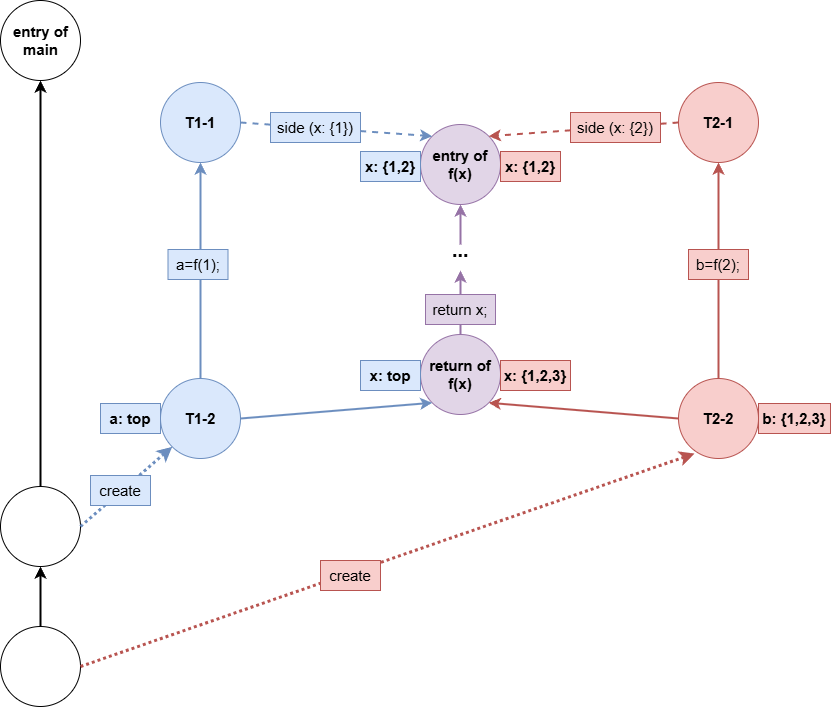
\includegraphics[width=\textwidth]{../resources/dist_no_fp.drawio.png}
    %  \end{subfigure}
    %  \caption[Example to show how the result of the disjoint \ac{td} might not satisfy the constraint system]{Example program (left) and simplified constraint system (right) to illustrate a case, where the result of the result of the disjoint \ac{td} might not satisfy the constraint system. Solid lines represent \texttt{query} edges, \texttt{side-effects} and \texttt{create} edges are labeled}
    %  \label{fig:example_noFP}
    %\end{figure*}
    %We consider the example in~\autoref{fig:example_noFP} to illustrate, how the result of the disjoint \ac{td} might not satisfy the constraint system after combining the mappings from the separate tasks. For this example, we consider an analysis, that tracks values of program variables in a set of values, a certain variable could hold at a given program point. The analysis is performed context insensitively. The solver starts the analysis from the end of the main function. It and follows the \texttt{query} edges and iterates the variables of the main function. During this, it triggers the \texttt{create} edges, initializing two separate tasks to compute a stable solution for the sub-systems corresponding to the threads \texttt{T1} and \texttt{T2}. The task that solves the sub-system of \texttt{T1} is shown in blue and the other one in red. Each of the two threads calls the function \texttt{f(x)} and assigns the return value of the call to a local program variable. Thus, both tasks of the solver have to analyze the function. Because the analysis is performed context insensitively, the tasks compute stable values for the same variables that correspond to the function \texttt{f(x)}. For both calls a side-effect is triggered to contribute the value of the argument to the entry variable of \texttt{f(x)}. Since the function is called with different arguments, the join of both contributions is used for the variable \textbf{entry of f(x)}. This results in the notion that the program variable \texttt{x} can be either 1 or 2 at this point. Furthermore, both tasks query the variable corresponding to the return state of 

    \paragraph{Sharing of side-effected variables} In the following we introduce a variant of the previously described disjunct \ac{td} that uses a shared data-structure to store the values of exactly those variables that receive side-effects. For this variant, we make use of the fact that in \gob\ all variables that receive side-effects only have a constant initial value as their \ac{rhs}. We call these variables \textit{side-effected variables}. These variables are only ever updated by side-effects and never through an iteration. Thus, we can have a \textit{lockable hash-table} inside the \texttt{Side} structure that directly contains the mapping from the side-effected variables to their value. The tasks of the solver do not contain this part of the mapping. When a side-effected variable is queried, the value is looked up in the central \texttt{Side} structure instead of the local solver mapping. When a side-effect is encountered by a task, it updates the shared mapping in the \texttt{Side} structure if the new value is not less or equal than the current one. If this is the case, it also adds the target variable to the list of side-effects. In this variant of the disjunct \ac{td} the values of the side-effects are not tracked in this list. This is because the other tasks only need to notice, which side-effected variables are updated but not the values of the updates. When a task checks the \texttt{Side} structure before evaluating a \ac{rhs} or before terminating, it looks up which side-effected variables were updated since it last checked and destabilizes those variables and all variables they influence. The main difference to the original disjunct \ac{td} is, that the processing of side-effects is moved from the individual tasks into the central \texttt{Side} structure. This avoids that all tasks perform the updates to side-effected variables individually. Ideally the sub-systems solved by the different tasks are disjunct, and thus each task only ever queries a subset of all side-effected variables. With the shared mapping in the \texttt{Side} structure, the tasks do not need to process and track the values of side-effected variables they never query.
    